\chapter{Entrenamiento de los agentes}

Una vez ya teníamos el entorno completado y testeado, la siguiente tarea consistía en entrenar a unos agentes en el entorno. Esto serviría como prueba de que el entorno es completamente funcional y además, como punto de referencia para futuras investigaciones en este entorno.

Antes de comenzar el entrenamiento, nos encontramos con varios problemas. En primer lugar, una forma habitual de realizar los entrenamientos es realizarlos en paralelo, creando diferentes instancias del entorno y entrenando a los agentes en ellos. El problema aparecía en que el entorno no estaba preparado para ser ejecutado en paralelo, puesto que usaba un puerto TCP fijo y además era necesario que implementara la librería EzPickle, que facilita la creación de entornos en paralelo. En segundo lugar, la instaciación del entorno era demasiado lenta y esto resultaba en un error al crearlos en paralelo. Para solucionar estos problemas tuvimos que optimizar la velocidad de carga del juego, además de realizar una comunicación a través de Pipes para conocer el puerto TCP que usara cada instancia del juego. Finalmente, se añadió el uso de la librería EzPickle para que crear entornos en paralelo fuera más sencillo.

\section{Introducción al método de entrenamiento}

Antes de explicar el proceso de entrenamiento, haremos una breve introducción al método que usaremos. Puesto que el objetivo de este apartado es solo entrenar un agente que sirva como modelo de referencia, solo daremos una idea intuitiva del método.

El método que usaremos para entrenar se llama \textbf{Proximal Policy Optimization (PPO)}. A este metodo le aplicaremos una \textbf{Convolutional neural network (CNN)}. Más tarde explicaremos cuál es el objetivo de cada uno de estos componentes.

\subsection*{Proximal Policy Optimization}

PPO es un algoritmo diseñado por el equipo Open IA en 2017 y rápidamente se convirtió en uno de los métodos de RL más populares superando incluso a otros métodos como Deep-Q learning. La idea básica detrás de PPO es que recoge un conjunto pequeño de experiencias o batch, y lo usa para actualizar la política de toma de decisiones. Una vez que se ha actualizado la política, las experiencias se desechan y se recogen nuevas usando la nueva política.

La principal contribución de PPO es que este se asegura que la nueva política de toma de acciones no ha cambiado demasiado con respecto a la política previa. Esto asegura que el entrenamiento es mucho más controlado y estable, consiguiendo así que el agente no sigue un camino de tomar acciones sin sentido.

\subsection*{Convolutional neural network}

CNN es una red de inteligencia artificial que se usa habitualmente para analizar imágenes. El objetivo de este usar este método es que CNN es capaz de a partir de una imagen, extraer la información relevante. Y gracias a esto se podrá entrenar al agente de forma eficiente. Realizar este paso en necesario, ya que si no se hiciera, la observación que los agentes deberían procesar es de 600 * 800 * 3 = 1440000 píxeles de información. Esto es realmente impracticable, por ello es necesario procesar la imagen y obtener los datos importantes de ella.

\subsection*{Entrenamiento}

Ahora que ya hemos explicado la idea intuitiva los métodos, nos quedaba la implementación. Para implementar esto, usamos la librería de stable baselines 3, que contiene una implementación sencilla y fácil de usar de PPO y CNN. Pero antes de esto se requería un cierto pre procesado del entorno. Para hacer este pre procesado utilizamos la librería SuperSuit. El objetivo de este pre procesado es disminuir el número de frames que utilizaran los agentes para entrenar. Aunque de esto ya se encarga CNN, podemos facilitar mucho el trabajo con unos simples pasos. 

Lo primero que hicimos fue reducir el color de las imágenes, que estaban en formato RGB, a únicamente el color azul. Solo con un color es suficiente para distinguir los diferentes elementos de una imagen. No se realiza un escalado a blanco y negro, ya que esto es computacionalmente más costoso. El siguiente paso fue reducir el tamaño de las imágenes de 600*800 a 84*84. Este tamaño de imagen fue escogido arbitrariamente, ya que es un tamaño usado habitualmente en otras investigaciones. Más tarde, decidimos compactar tres frames del entorno en uno solo. Esto se hace porque de esta manera es más sencillo para el agente entender el movimiento que ocurre en el entorno. Finalmente añadimos un envoltorio a nuestro entorno modificado para que este pudiera ser ejecutado en paralelo y comenzamos el entrenamiento de los agentes. PPO tiene varios hyperparametros que se pueden tunear. Decidimos realizar aleatoriamente diferentes configuraciones de hyperparametros, pero puesto que ninguna parecía dar resultados distintos, decidimos usar como versión final los hyperparametros por defecto. Para el entrenamiento decidimos realizar 500000 iteraciones, que tomaron aproximadamente 7 horas en completarse.

\subsection*{Conclusiones}

A modo de conclusión, después de todo el entrenamiento, los agentes no son capaces de solucionar el primer obstáculo del primer nivel. Creemos que esto se debe a varias razones. La primera de todas es que el modelo de entrenamiento no está eficientemente tuneado. También creemos que se debe a que el entorno que deben solucionar es realmente duro. Observemos de nuevo el primer obstáculo del primer nivel. Este lo podemos ver en la figura \ref{fig:mapa-duro}.

\begin{figure}[ht]
    \centering
    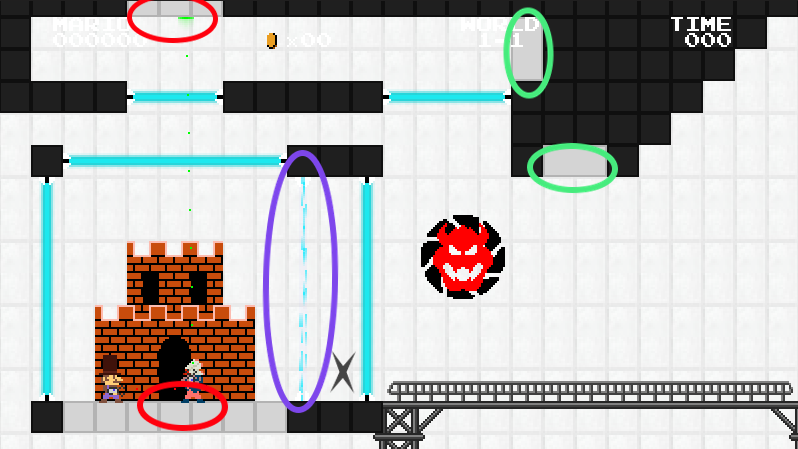
\includegraphics[width=0.9\textwidth]{img/mario-1-level.png}
    \caption{Primer nivel del mapa Bowser Cooperative Testing Initiative \cite {mari0-mapa}}
    \label{fig:mapa-duro}
\end{figure}

En el apartado de Mapa cooperativo ya explicamos los pasos necesarios para resolver este primer obstáculo, aun así, vamos a repetir en este apartado los pasos para valorar que recompensas obtendrían los agentes.

La forma de resolver este nivel es la siguiente:
\begin{itemize}
    \item \textbf{Paso 1}: En primer lugar, uno de los dos jugadores, de ahora en adelante jugador 1, debe colocar un portal en cada uno de los círculos rojos indicados en la figura. Con este movimiento se consigue que el jugador 1 pase a la sección superior. Durante la ejecución de esta acción, los agentes no obtienen ninguna recompensa, ya que el jugador 2 se queda dentro del cuadrilátero, por ello se convierte en el jugador más cercano al punto de inicio y por lo tanto no obtiene puntos al no alejarse este.
    \item Paso 2: El jugador 2 debe colocarse donde se encuentra la X indicada en la figura. Desde esta posición debe disparar dos portales a los círculos verdes indicados en la figura. Con este paso el jugador 1, que se encuentra en la sección superior, será capaz de atravesar estos portales y pasar fuera del cuadrilátero inicial. Gracias a esta acción, solo se consigue las recompensas del movimiento que ha realizado el jugador 2 hacia la X indicada en la figura. Aunque el jugador 1 ha avanzado claramente, ninguna de acciones tienen recompensa.
    \item Paso 3: Una vez el jugador 1 se encuentra fuera del cuadrilátero, el jugador 2 deberá realizar las mismas acciones que el jugador 1 en el primer paso. De nuevo, el jugador 2 debe realizar un conjunto de acciones que en principio no le otorgaran ninguna recompensa hasta que consiga subir a la sección superior. Suponiendo que consiga ejecutar este paso, sí se le otorgará la recompensa correspondiente.
    \item Paso 4: Mientras eso ocurre, el jugador 1 deberá colocar sus portales donde los colocó el jugador 2 en el paso 2. Esta acción en sí no aporta ninguna recompensa al agente por lo que al entorno respecta, la única recompensa recibida se debe a que el jugador 1 se ha desplazado por la sección superior en el paso anterior.
    \item Si se han realizado correctamente todos los pasos, ambos jugadores deberían haber salido del cuadrilátero inicial. Finalmente cuando ambos jugadores hayan conseguido salir, se les otorgara la recompensa de poder seguir avanzando por el nivel.
\end{itemize}

Como hemos visto, los agentes deben de tomar varias decisiones que no les aportan ninguna recompensa para obtener una recompensa mayor y poder avanzar. Esto es habitual en la mayoría de entornos de RL, pero el set de acciones que estos deben de realizar no es trivial y por lo tanto puede dificultar bastante el aprendizaje de los agentes. Por estas razones creemos que aun después del entrenamiento, los agentes no han conseguido resolver el problema. Sin embargo, esto no debe desalentar, ya que el objetivo no era solucionar el entorno. De hecho esto presenta una obstáculo a resolver en otras investigaciones.